% Figure 1 — multi-scale linear-attention encoder, end to end.
% Standalone: pdflatex fig_overview_tikz.tex -> fig_overview_tikz.pdf.
% txfonts = the fonts elsarticle's `times` option loads.
%
% Every icon is built only from rectangles, lines and circles, so the plate can
% be re-laid out by moving a coordinate rather than redrawing an illustration.
% Palette tokens are shared with Figures 2 and 3.
\documentclass[border=2pt]{standalone}
\usepackage[T1]{fontenc}
\usepackage{amsmath}
\usepackage{txfonts}
\usepackage{tikz}
\usetikzlibrary{positioning, arrows.meta, calc}

\definecolor{fink}{HTML}{2B3A45}
\definecolor{sandF}{HTML}{F2EFEA}
\definecolor{sandL}{HTML}{7A6F5F}
\definecolor{slate1}{HTML}{E9EEF2}
\definecolor{slate2}{HTML}{D6E0E8}
\definecolor{slate3}{HTML}{C3D0DB}
\definecolor{slateL}{HTML}{4E6371}
\definecolor{brassF}{HTML}{EFDCC6}
\definecolor{brassL}{HTML}{8B6636}
\definecolor{veilF}{HTML}{FBFAF8}

\tikzset{
  arr/.style  = {->, >={Stealth[length=1.6mm]}, semithick, fink!85},
  bus/.style  = {semithick, fink!85},
  dim/.style  = {<->, >={Stealth[length=1.3mm]}, semithick, brassL},
flow/.style = {->, >={Stealth[length=1.3mm]}, semithick, brassL, dashed},
  cell/.style = {very thin, black!40},
  capx/.style = {font=\footnotesize, text=fink!85, align=center},
  head/.style = {font=\footnotesize, text=fink},
  note/.style = {font=\scriptsize, text=fink!85, align=center},
  bare/.style = {font=\scriptsize, text=fink!80},
  rule/.style = {black!30, thin},
}

\begin{document}
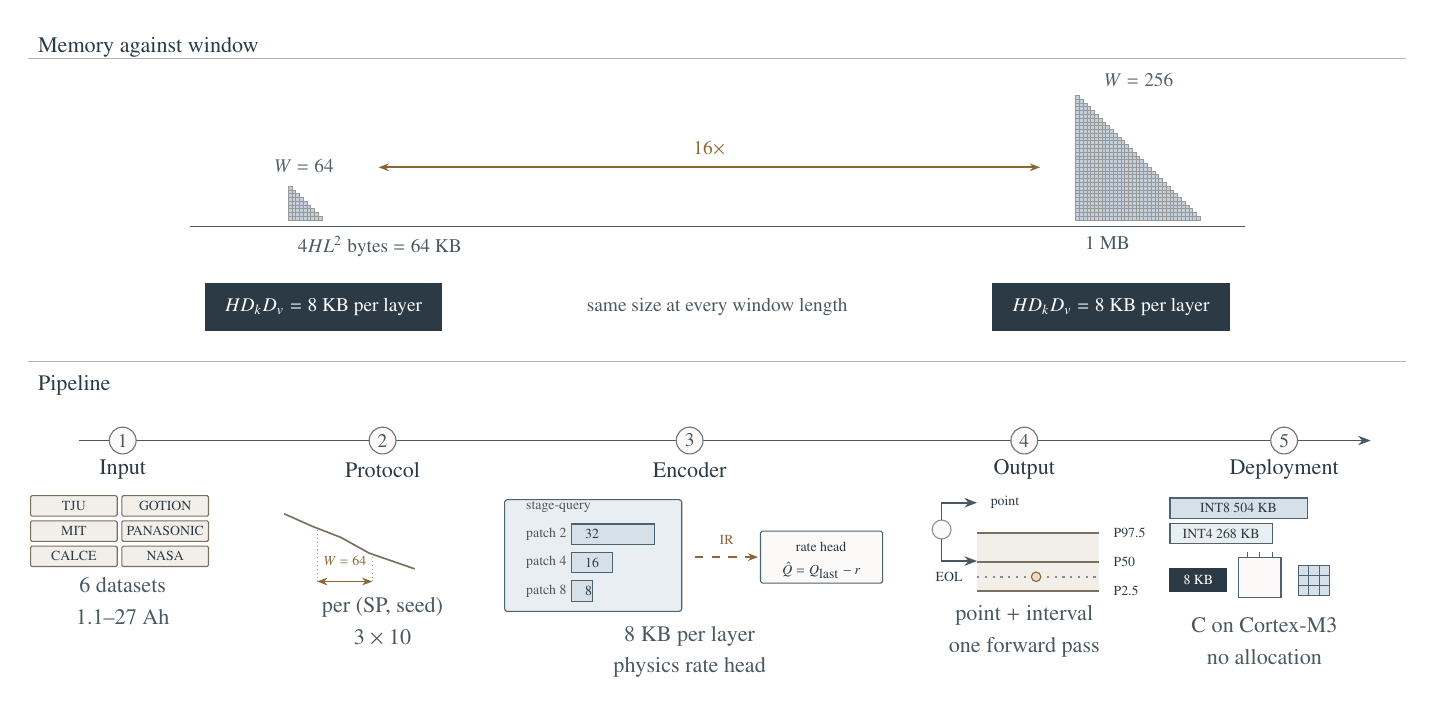
\begin{tikzpicture}

% GRID
%   rows   : 10.15 header | 10.00 rule | 9.65-7.95 grids | 7.85 labels |
%            7.15-6.55 state | 6.15 rule | 5.85 header | 5.15 numbers |
%            4.78 names | 4.45-2.95 glyphs | 2.85 captions
%   cols   : 0.25-2.65 input | 3.45-6.05 protocol | 6.30-11.00 encoder |
%            11.40-14.40 output | 14.70-17.75 deployment

\node[head, anchor=west] at (0.25,10.15) {Memory against window};
\draw[rule] (0.25,10.00) -- (17.75,10.00);

% ---- grids: identical cell size, one baseline at 7.95
\foreach \n/\x in {8/3.55, 32/13.55}{
  \foreach \r in {0,...,\n}{
    \pgfmathsetmacro{\ry}{\n-\r}
    \foreach \c in {0,...,\r}{
      \draw[cell, fill=slate3] (\x+\c*0.048,7.95+\ry*0.048) rectangle ++(0.048,0.048);
    }}}
\node[bare, anchor=south] at (3.75,8.42) {$W=64$};
\node[bare, anchor=south] at (14.35,9.52) {$W=256$};
\node[note, anchor=north west] at (3.55,7.87) {$4HL^{2}$ bytes $=64$ KB};
\node[note, anchor=north west] at (13.55,7.87) {$1$ MB};
\draw[bus] (2.30,7.87) -- (15.70,7.87);
\draw[dim] (4.70,8.62) -- (13.10,8.62);
\node[note, text=brassL, anchor=south] at (8.90,8.66) {$16\times$};

% ---- state: two identical blocks; their equal size is the statement
\foreach \x in {2.50,12.50}{
  \draw[fink, fill=fink] (\x,6.55) rectangle ++(3.00,0.60);
  \node[font=\scriptsize, text=white] at (\x+1.50,6.85) {$HD_kD_v = 8$ KB per layer};
}
\node[note] at (9.00,6.85) {same size at every window length};

\draw[rule] (0.25,6.15) -- (17.75,6.15);
\node[head, anchor=west] at (0.25,5.85) {Pipeline};

\draw[arr] (0.90,5.15) -- (17.30,5.15);
\foreach \x/\i in {1.45/1, 4.75/2, 8.65/3, 12.90/4, 16.20/5}{
  \draw[fill=veilF, draw=fink!70] (\x,5.15) circle (0.17);
  \node[note] at (\x,5.15) {\i};
}
\foreach \x/\t in {1.45/Input, 4.75/Protocol, 8.65/Encoder, 12.90/Output, 16.20/Deployment}{
  \node[head] at (\x,4.78) {\t};
}

% ---- 1 input: two rows of three chips inside 0.25-2.65
\foreach \k/\name in {0/CALCE, 1/NASA, 2/MIT, 3/PANASONIC, 4/TJU, 5/GOTION}{
  \pgfmathsetmacro{\col}{mod(\k,2)}
  \pgfmathsetmacro{\row}{int(\k/2)}
  \draw[draw=sandL, fill=sandF, rounded corners=0.5pt]
    (0.28+\col*1.16, 3.55+\row*0.32) rectangle ++(1.10,0.26);
  \node[font=\tiny, text=fink] at (0.83+\col*1.16, 3.68+\row*0.32) {\name};
}
\node[capx, anchor=north] at (1.45,3.54) {6 datasets\\[2pt]1.1--27 Ah};

% ---- 2 protocol
% a short capacity trace with one window marked on it
\draw[sandL, semithick] (3.50,4.22) -- (3.86,4.06) -- (4.22,3.92)
                         -- (4.58,3.72) -- (5.16,3.52);
\draw[fink!45, densely dotted] (3.92,3.36) -- (3.92,4.05);
\draw[fink!45, densely dotted] (4.62,3.36) -- (4.62,3.73);
\draw[dim] (3.92,3.36) -- (4.62,3.36);
\node[font=\tiny, text=brassL, anchor=south] at (4.27,3.44) {$W=64$};
\node[capx, anchor=north] at (4.75,3.28) {per (SP, seed)\\[2pt]$3\times10$};

% ---- 3 encoder: three parallel branches, bar length is the token count
\draw[draw=slateL, fill=slate1, rounded corners=1pt] (6.30,2.98) rectangle ++(2.25,1.42);
\node[font=\tiny, text=fink!85, anchor=west] at (6.45,4.30) {stage-query};
\foreach \lab/\tok/\len/\yy in {patch 2/32/1.05/3.96, patch 4/16/0.525/3.60, patch 8/8/0.2625/3.24}{
  \node[font=\tiny, text=fink!85, anchor=west] at (6.45,\yy) {\lab};
  \draw[draw=slateL, fill=slate2] (7.15,\yy-0.13) rectangle ++(\len,0.26);
  \node[font=\tiny, text=fink, anchor=west] at (7.20,\yy) {\tok};
}



% rate head, fed by measured IR
\draw[draw=slateL, fill=veilF, rounded corners=0.6pt] (9.55,3.34) rectangle ++(1.55,0.66);
\node[font=\tiny, text=fink] at (10.32,3.80) {rate head};
\node[font=\tiny, text=fink] at (10.32,3.50) {$\hat{Q}=Q_{\text{last}}-r$};
\draw[flow] (8.72,3.67) -- (9.52,3.67);
\node[font=\tiny, text=brassL, anchor=south] at (9.12,3.71) {IR};
\node[capx, anchor=north] at (8.65,2.92) {8 KB per layer\\[2pt]physics rate head};

% ---- 4 output: point on top, calibrated interval below
\draw[fill=veilF, draw=fink!55] (11.85,4.02) circle (0.12);
\draw[arr] (11.85,4.14) -- (11.85,4.36) -- (12.30,4.36);
\node[font=\tiny, text=fink, anchor=west] at (12.35,4.36) {point};
\draw[arr] (11.85,3.90) -- (11.85,3.62) -- (12.30,3.62);
\draw[fill=sandF, draw=none] (12.30,3.24) rectangle (13.85,3.98);
\foreach \yy in {3.24,3.61,3.98}{\draw[sandL, semithick] (12.30,\yy) -- (13.85,\yy);}
\foreach \yy/\l in {3.98/P97.5, 3.61/P50, 3.24/P2.5}{
  \node[font=\tiny, text=fink, anchor=west] at (13.91,\yy) {\l};
}
\draw[black!45, dotted, thick] (12.30,3.42) -- (13.85,3.42);
\node[font=\tiny, text=fink, anchor=east] at (12.24,3.42) {EOL};
\draw[fill=brassF, draw=brassL] (13.05,3.42) circle (0.06);
\node[capx, anchor=north] at (12.90,3.18) {point $+$ interval\\[2pt]one forward pass};

% ---- 5 deployment
\draw[draw=slateL, fill=slate2] (14.75,4.16) rectangle ++(1.75,0.26);
\node[font=\tiny, text=fink] at (15.62,4.29) {INT8 504 KB};
\draw[draw=slateL, fill=slate1] (14.75,3.84) rectangle ++(1.30,0.26);
\node[font=\tiny, text=fink] at (15.40,3.97) {INT4 268 KB};
\draw[fink, fill=fink] (14.75,3.24) rectangle ++(0.72,0.28);
\node[font=\tiny, text=white] at (15.11,3.38) {8 KB};
\draw[draw=slateL, fill=veilF] (15.62,3.16) rectangle ++(0.54,0.50);
\foreach \k in {0,1,2}{\draw[slateL] (15.73+\k*0.16,3.66) -- ++(0,0.07);}
\foreach \i in {0,1,2}{\foreach \j in {0,1,2}{
  \draw[very thin, slateL, fill=slate2]
    (16.38+\i*0.13,3.18+\j*0.13) rectangle ++(0.13,0.13);}}
\node[capx, anchor=north] at (15.95,3.02) {C on Cortex-M3\\[2pt]no allocation};

\end{tikzpicture}
\end{document}
